%% eval.tex
%% $Id: eval.tex 5 2005-10-10 20:55:48Z bless $

%%%%%%%%%%%%%
ion\chapter{Evaluation}
\label{ch:evaluation}
%%%%%%%%%%%%%

Zur Gegenüberstellung und Evaluation der entwickelten Ansätze, wurde eine Studie entwickelt und durchgeführt. In diesem Kapitel wird zunächst das Studiendesign, der genau Hergang der Studie sowie die zu evaluierenden Hypothesen erläutert. Anschließend werden die erhobenen Daten beschrieben. Die Betrachtung und Diskussion der Daten erfolgt anschließend in Kapitel \ref{ch:Results}. 

\section{Studie}
Basierend auf den entwickelten Konzepten, wurde eine Studie entwickelt um diese zu evaluieren. Zweck der Studie, Probandenakquise, Studiendesign und Studienablauf werden nachfolgend beschrieben. Darüber hinaus werden die zu untersuchenden Hypothesen näher erläutert. 

%Basierend auf einer ausgewählten Probandengruppe, ist es für die Überprüfung der aufgestellten Hypothesen bedeutend, die jeweiligen Probanden zu framen. Hierfür werden zunächst Sinn der Studie und diverse Begriffe erläutert. Anschließend machen sich die Probanden mit dem jeweiligen Programm vertraut, welches betrachtet werden soll. Hierfür wird eine Aufgabe gestellt, die durch das Programm führt und den Probanden beim explorieren des jeweiligen Programms und dessen Funktionen anleitet. Während der Nutzung und der Bearbeitung der gestellten Aufgaben, werden Emotionen und Motivationen durch Kommentare des Probanden erfasst. Abschließend wird nach der aufgabengesteuerten Nutzung eines Programms eine erste Einschätzung in Form eines Fragebogens erfasst. Nach Bearbeitung aller Aufgaben und Verwendung beider Programme, werden die Programme in einer abschließenden Fragerunde miteinander verglichen. Dabei wird auf wesentliche Unterschiede beider Programme eingegangen. Erfasst werden hierbei die Einschätzung der Probanden, welche Eigenschaften sie im Vergleich als besonders Hilfreich, nicht Hilfreich empfanden. Auch welche Eigenschaften ihnen gefallen oder welche sie vermisst haben. Diese Einschätzungen werden in Relation zu den Ergebnissen der Fragebögen gesetzt um diese zu verargumentieren. 


\subsection{Zweck der Studie}
Ziel der Studie ist die Bewertung verschiedener Konzepte, die im Rahmen des entwickelten Modellierungsansatz umgesetzt wurden. Als Baseline dient hierbei das in Kapitel \todo{Verweis auf movisensXS Kapitel} vorgestellte System \emph{movisensXS}. Dieses Tool wird bereits, mit größerem Funktionsumfang, in der Psychologie für \emph{Experience Sampling} verwendet. Anhand der Konzeption dieses Produkts können bereits Chatbot-ähnliche Anwendungen generiert werden. Untersucht werden das Konstruktionsprinzip, Konfigurationsprinzip, Sprünge und Sichtbarkeitsregeln. Dabei soll in der Studie auf die Unterschiede zwischen Konstruktionsprinzip und Konfigurationsprinzip sowie Sprüngen und Sichtbarkeitsregeln eingegangen werden. Anschließend sollen die einzelnen Konzepte bewertet und die Ergebnisse gegenüber gestellt werden. Herausgefunden werden soll welche der Konzepte, zur Erstellung eines Chatbots, eine höhere Akzeptanz haben, weshalb diese besser bewertet werden und welche Probleme sie in diesen Konzepten sehen. 

\subsection{Probandenakquise}


\subsection{Studiendesign}
Es wurde eine formative Laborstudie, mit einer Gruppe von acht Probanden, durchgeführt. Beobachtet wurde der Umgang eines Probanden mit  zwei Prototypen. Durchgeführt wurde die Studie jeweils mit einem Probanden und einem Studienleiter in einem vorbereiteten Labor. Jedem Probanden wurden zunächst ein Vorfragebogen vorgelegt und anschließend vier Hauptaufgaben gestellt, die sich jeweils in weitere Unteraufgaben teilen. Je zwei Hauptaufgabenstellungen beziehen sich auf einen Prototyp. 
Die Aufgaben beinhalten \emph{Think Aloud} und \emph{Screen Recording}. Die Reihenfolge der Aufgabenstellung wurde nach dem \emph{counterbalancing-measures-Design} gestellt und variierten somit zwischen 1,2,3,4 und 3,4,1,2. Aufgaben 1 und 2 betreffen den erstellten Prototypen. Die Aufgaben 3 und 4 betreffen die \emph{movisensXS} Konfiguration. Während der Proband die Aufgaben bearbeitete, unterstützte der Studienleiter den Proband bei der Aufgabenbearbeitung, stellte gezielt Fragen und erstellte eine Video-Aufnahme des Studienverlaufs. Nachdem die Aufgaben zu einem Prototyp bearbeitet wurden, füllte der Proband abschließend einen Fragebogen zum entsprechenden Prototyp aus. Wurden alle Aufgaben bearbeitet führte der Studienleiter mit dem Proband eine Abschlussfragerunde durch.

\subsection{Studienablauf}
Zunächst bereitete der Studienleiter das Setting in einem ruhigen Raum, mit Internet- und Stromanschluss, vor. Hierfür ging er eine Checkliste durch, um sich zu vergewissern, dass alle benötigten Geräte, Hilfsmittel, Programme und Unterlagen vorhanden, funktionsfähig und korrekt eingestellt sind. Anschließend wurde die Nummer des Probanden notiert. Anhand dieser Nummer wurden die Aufgabenblätter nach ihrer Bearbeitungsabfolge vorbereitet.

Sobald der Studienleiter das Setting der Studie vorbereitet und überprüft hatte, wurde der Proband begrüßt und in den Raum gebeten. Wie in Abbildung \ref{studienablauf} zu sehen ist, wurde zunächst der grobe Studienablauf erklärt. Auch wurde darauf eingegangen, welche Daten erhoben werden und wie die Aufzeichnung dieser stattfindet. Der Studienleiter vergewissert sich anschließend, ob seitens des Probanden noch offene Fragen bestehen. Bestehen keine Fragen, wurde dem Probanden die Datenschutzerklärung und Einverständniserklärung vorgelegt. Diese sollte er sich in Ruhe durchlesen und, bei Einverständnis, unterschreiben. Nach Unterzeichnung der Dokumente, erklärte der Studienleiter den genauen Ablauf der Studie und die Aufgaben, die an den Probanden gestellt werden. Außerdem wurde der Proband gebeten, laut und deutlich seine Gedankengänge zu äußern, während er die Aufgabe bearbeitet.

Sofern keine weiteren Fragen zum Studienablauf und der Aufgabenbearbeitung bestanden, startete der Studienleiter den Screen Recorder und die Kamera, um den Probanden, sowie den Bildschirm des Laptops, in Bild und Ton aufzunehmen. Des Weiteren wurde dem Probanden das erste Aufgabenblatt zur Bearbeitung vorgelegt. Wie in Abbildung \ref{studienablauf} zu sehen ist, erfolgte zunächst eine Überprüfung um die Aufgabe festzulegen, mit der gestartet werden soll. Lief der Proband unter einer geraden Nummer, so erhielt er zuerst die Aufgaben drei und vier, zum angepassten \emph{movisensXS} System. Wurde der Proband einer ungeraden Nummer zugeteilt, so begann dieser mit den Aufgaben eins und zwei, die sich auf den \emph{TherapyBuilder}-Prototyp beziehen. 

Wurde das erste Aufgabenblatt bearbeitet, so erhielt der Proband einen Fragebogen zum eben bearbeiteten System. Anschließend überreichte der Studienleiter dem Proband das nächste Aufgabenblatt. Im Falle einer geraden Probandennummer wurden nachfolgend die Aufgaben eins und zwei bearbeitet. Andernfalls die Aufgaben drei und vier. Auch nach Abschluss dieser Aufgaben folgte ein Fragebogen zum soeben genutzten System. Wurde dieser ausgefüllt, folgte abschließend eine Fragerunde. Der Studienleiter erläuterte die vier verwendeten Konzepte \emph{Konstruktionsprinzip}, \emph{Konfigurationsprinzip}, \emph{Sprünge} und \emph{Sichtbarkeitsregeln}. Daraufhin folgte die Befragung des Probanden. Dieser sollte zunächst darauf eingehen was er an den jeweiligen Konzepten \emph{hilfreich} und \emph{nicht hilfreich} empfunden hat. Außerdem sollte er erklären was ihm besonders gut an dem jeweiligen Ansatz \emph{gefallen} und welche Eigenschaften ihm \emph{gefehlt} haben. 

\begin{figure}[h]
\centering
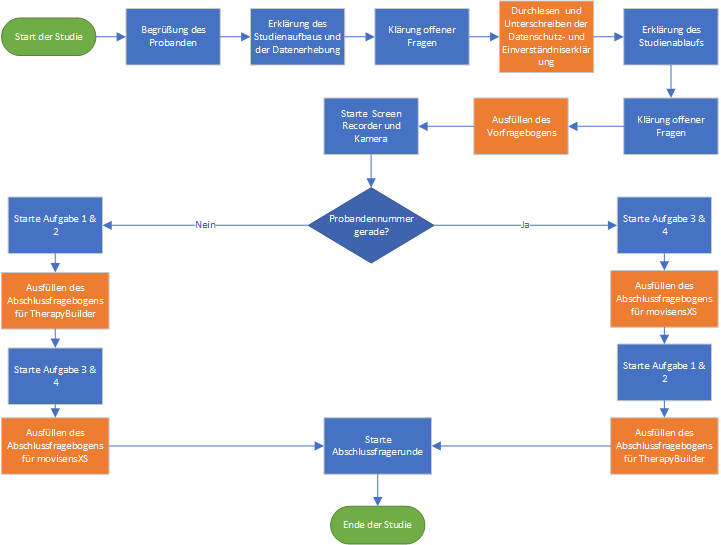
\includegraphics[width=1\textwidth]{pictures/diagramme/studienablauf-diagramm}
\caption{Ablauf der Studie. Orange kennzeichnet die Aktionen des Probanden. Blau stellt die Aktionen des Studienleiters dar.}
\label{studienablauf}
\end{figure}


\subsection{Hypothesen}

\section{Beschreibung des erhobenen Datensatzes}
Nach der Durchführung der Studie gilt es, die Datensätze dieser auszuwerten und einzuordnen. Hierfür werden mehrere erhobenen Daten betrachtet. Die Evaluation der Studienergebnisse besteht zunächst aus der Beschreibung der Charakteristika der Probandengruppe. Anschließend werden die Ergebnisse der Erhebungen beschrieben. Eingegangen wird hierbei auf die Ergebnisse der Fragebögen, sowie der Abschließenden Fragerunde der untersuchten Konzepte.  


\subsection{Charakteristika der Probandenstichproben}
Es nahmen acht Probanden an der Vergleichsstudie teil. Diese befinden sich zum Zeitpunkt der Durchführung im Alter von 23 bis 37 Jahren. Das durchschnittliche Alter beträgt 29. Die Probandengruppe setzt sich aus fünf Frauen und 3 Männern zusammen. Die Probanden sind wissenschaftliche Mitarbeiter, Promotionsstudenten oder Doktoren aus dem medizinischen Bereich. 

Folgende Aussagen lassen sich über die Gewohnheiten und Technologienutzung der Probanden ableiten. Die Mehrheit verwendet ein- oder mehrmals am Tag Chat-Technologien. Ein Proband nutzt Chat-Technologien 
einmal im Monat oder seltener. Die verwendeten Chat-Technologien setzen sich aus Whatsapp, Telegram, Facebook Messenger, Instagram, Threema, Apple Nachrichten, Line und Slack zusammen. Die meistgenutzten Chat-Technologien innerhalb der Probandengruppe sind Whatsapp und Facebook Messenger. Verwendet werden diese Anwendungen hauptsächlich auf dem Smartphone oder Laptop bzw. Desktop Computer. 

Die Nutzung von Chatbots ist innerhalb der Probandengruppe wenig verbreitet. Diese werden von zwei Probanden einige Male pro Woche und einmal im Monat oder weniger genutzt. Genutzt werden der Nachrichtenbot der Tagesschau und ein Chatbotdienst für den Kundenservice der Firma ASOS. Bedient werden diese Chatbotdienste auf dem Smartphone sowie Laptop bzw. Desktop Computer. 

Innerhalb der Probandengruppe wurde Experience Sampling bereits mehrheitlich genutzt. Drei Probanden gaben an noch nie oder nur gelegentlich Experience Sampling verwendet zu haben. Fünf Probanden haben bereits Experience Sampling öfters bis regelmäßig genutzt. Für Experience Sampling kamen die Anwendungen movisensXS, Menthal und Whatsanalyzer zum Einsatz. Genutzt wurden diese auf dem Smartphone oder Laptop bzw. Desktop Computer. 

Hinsichtlich der Vorerfahrungen bezüglich movisensXS lassen sich für die Probandengruppe folgende Aussagen treffen. Wie in Grafik \ref{movisensXSErfahrung} zu sehen ist, besitzt ein Proband keinerlei Erfahrungen mit movisensXS. Die restlichen Probanden nutzen das Programm gelegentlich bis regelmäßig. Die Nutzung von movisensXS beschränkt sich auf das Zuordnen von Probanden, Teilnahme an Studien, sowie kleinen Anpassungen einer bereits bestehenden Studie. 

\begin{figure}[h]
\centering
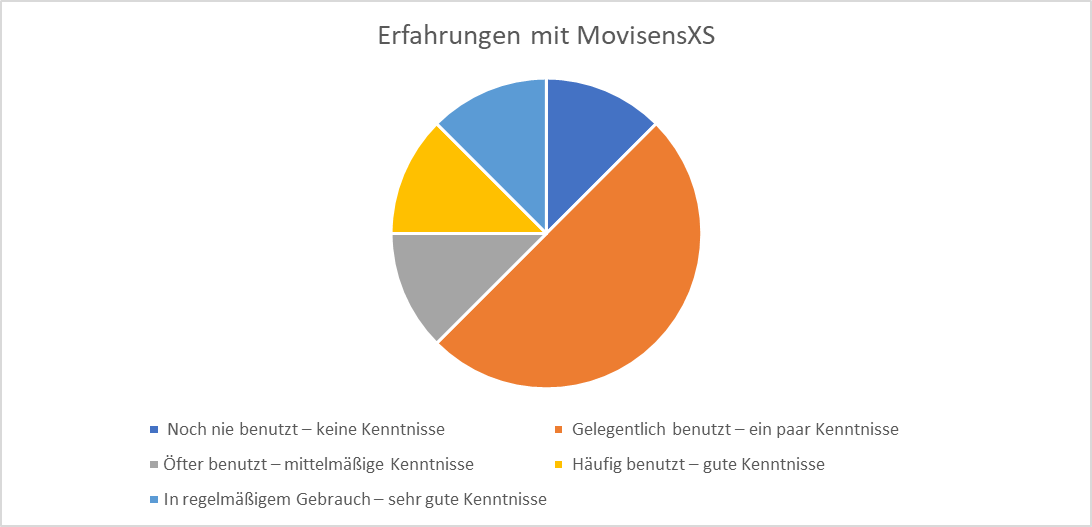
\includegraphics[width=1\textwidth]{pictures/diagramme/movi}
\caption{Angaben der Probanden bezüglich ihrer Erfahrungen mit dem Programm \emph{movisensXS}}
\label{movisensXSErfahrung}
\end{figure}

%%%%%%%%%%%%%%%%%%%%%%%%%%%%%%%%%%%%%%%%%%%%%%%%%%%%%%%%%%%%%%%%%%%%%%%%%%%%%%%%%%%%%%%%%%%%%%%%%%%%%% NEW order
%%%%%%%%%%%%%%%%%%%%%%%%%%%%%%%%%%%%%%%%%%%%%%%%%%%%%%%%%%%%%%%%%%%%%%%%%%%%%%%%%%%%%%%%%%%%%%%%%%%%%%

\subsection{Evaluationsergebnis des Konstruktionsprinzips}
Das Konstruktionsprinzip bietet das Einstellen der Trigger durch das Zusammensetzen und Verschalten einzelner Blöcke mit unterschiedlichen Funktionen. Wie in Abbildung \ref{konstruktion} dargestellt, bildet sich aus der Anordnung ein Baum aus verschiedenen Blöcken. Die Blöcke unterscheiden sich farblich und folgen dem Ampelprinzip.  

\begin{figure}[h]
\centering
\includegraphics[width=1\textwidth]{pictures/konstruktion}
\caption{Das Konstruktionsprinzip des movisensXS. Blöcke werden miteinander verschaltet.}
\label{konstruktion}
\end{figure}

Nachfolgend werden die erhobenen Daten beschrieben, die bezüglich des Konstruktionsprinzips erhoben wurden. Zunächst werden die Ergebnisse des Zwischenfragebogens, anschließend die Ergebnisse der Abschlussfragerunde dargestellt.

\subsubsection{Zwischenfragebogen}
Die Probanden gaben nach der Aufgabenbearbeitung an, dass sie die Darstellung der Trigger als zumeist verständlich empfanden mit einer leichten Tendenz zu zum Teil verständlich. Dies wird auch durch die Freitext-Aussagen der Probanden gestützt. Fünfundsiebzig Prozent der Probanden gingen auf die positive Auswirkung der farblichen Kodierung ein. Zum einen wurde beschrieben, dass diese die Orientierung innerhalb des Baumes erleichtern und die Funktion sowie Abfolge der Bausteine gut beschreiben.

Die Verständlichkeit der Einstellungsmöglichkeiten der Trigger wurde von den Probanden sehr unterschiedlich bewertet. Im Schnitt wird diese als zum Teil verständlich und zumeist verständlich empfunden. Positiv wurde von einem Probanden die vielen möglichen Trigger-Optionen hervorgehoben.

Während des Durcharbeitens der Aufgaben wurden die Probanden in der Trigger-Ansicht mit Verzweigungen zwischen einzelner Konversationen konfrontiert. Diese wurden im movisensXS als zum Teil verständlich empfunden. Diese Auswertung findet sich auch in den Aussagen wieder. Die Hälfte der Probanden gibt an, dass die Baumdarstellung bei vielen Bausteinen schnell unübersichtlich wirkt. 

Innerhalb des Baumes kann abgeleitet werden, welche Konversationen im Laufe des Therapiemoduls gestartet werden. Das Auffinden dieser Konversationen bewerteten die Probanden als eher gut. Dies findet sich auch in der bereits erwähnten Aussage der Probanden über die Unübersichtlichkeit der Darstellung wieder. 

Auch empfanden es die Probanden als eher schwierig die zeitliche Abfolge der Konversationen nachzuvollziehen. Im Schnitt bewerteten sie auch diese eher gut mit leichter Tendenz zu mäßig. Ein Proband beschrieb, dass der Baum nicht auf den ersten Blick erkennen lässt, was dieser Bedeutet. Ein weiterer merkte an, dass die Darstellung für den entsprechenden Zweck nicht sehr intuitiv ist. 

Das Anordnen der Bausteine zur Konfiguration der Trigger empfanden die Probanden im Schnitt gut verständlich. Dies wurde auch von den Probanden positiv hervorgehoben. Zwei Probanden beschreiben, dass das Baukasten-Prinzip die Konfiguration erleichtert. Ein Proband weißt ebenfalls auf die bereits erwähnte Vielfalt der Trigger-Optionen hin. Darüber hinaus wurde von knapp achtunddreißig Prozent die Anordnung der Bausteine via Drag and Drop positiv hervorgehoben.

Die Abhängigkeiten ließen sich hingegen nicht so gut erkennen. Im Schnitt tendiert die Einschätzung der Probanden eher zu einer eher guten Darstellung der Abhängigkeiten zwischen verschiedenen Konversationen. Dies kann erneut mit der, von den Probanden mehrfach genannten, Unübersichtlichkeit in Verbindung gebracht werden. 

Insgesamt empfanden die Probanden die Übersichtlichkeit der Therapie und deren Verlauf als eher mäßig. Ein Proband gab an, dass die Therapie für ihn schlecht zu überschauen ist. Die restlichen Probanden hingegen bewerteten diese zwischen sehr gut bis eher gut. Dies spiegelt sich wiederum in der Aussage über die fehlende Übersichtlichkeit innerhalb der Baum-Darstellung wieder. Dies wurde - wie bereits erwähnt - von fünfzig Prozent der Probanden angemerkt. 

\subsubsection{Abschlussfragerunde}
Die Abschlussfragerunde ergab sechzig Aussagen. Achtzehn Prozent der Aussagen bezogen sich auf die Frage, welche Eigenschaften dieser Form der Umsetzung, als besonders Hilfreich erfahren wurden. Auf die Frage hin, welche Eigenschaften als hinderlich empfunden wurden, konnten fünfunddreißig Punkte genannt werden. Diese machen fünfunddreißig Prozent der Abschlussfragerunde aus. Hingegen bezogen sich achtundzwanzig Prozent der Aussagen auf die Frage was den Probanden an dieser Form der Umsetzung besonders gut gefallen hat. Elf Punkte wurden von den Probanden genannt, die sie am System vermisst haben. Dies macht ebenfalls achtzehn Prozent der Aussagen über die Umsetzung aus. 

\begin{figure}[h]
\centering
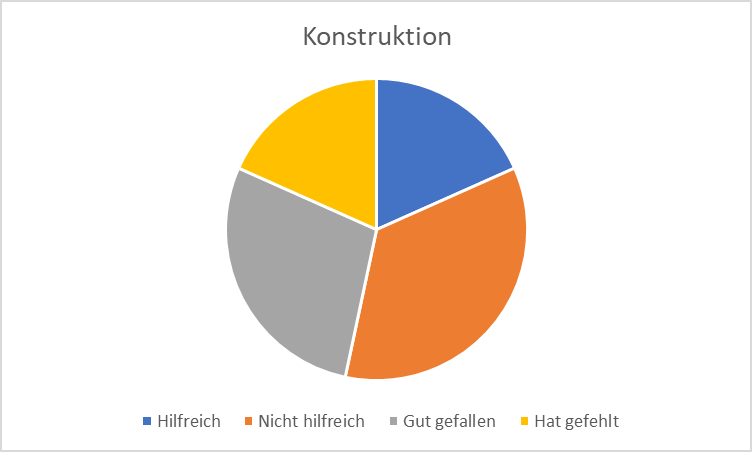
\includegraphics[width=1\textwidth]{pictures/diagramme/aussagenkonstr}
\caption{Anteile der Aussagen, die Probanden in der abschließenden Fragerunde bezüglich des verwendeten Konstruktionsprinzips äußerten.}
\label{aussagensichtb}
\end{figure}


\paragraph{Hilfreich}Zwei Probanden konnten keine Antwort auf die Frage geben, was sie an dieser Umsetzungsform besonders hilfreich empfanden. Sechsunddreißig Prozent der Antworten gaben an, dass sie insbesondere die farbliche Kodierung der Bausteine als besonders hilfreich empfanden. Somit konnten Beziehungen zwischen Bausteinen besser nachvollzogen werden. Eine weitere Anmerkung eines Probanden unterstützt diese Erklärung. So sagte dieser aus, dass die Farben dabei halfen, sich im Baum zu orientieren. Rote Elemente befinden sich oben, gelbe in der Mitte und Grüne befinden sich in der Darstellung unten. Dies unterstützt bei der Orientierung. Siebenundzwanzig Prozent der Probanden äußerten, dass die grafische Darstellung hilfreich war. So hatten diese mehr Infos auf einem Blick und konnte die Abhängigkeiten gut einsehen. Achtzehn Prozent der Probanden gingen auf die Navigation innerhalb des Prototyps ein. So empfanden sie die Navigation zur Baum-Darstellung als hilfreich. Diese war klar und half dabei sich schneller zurecht zu finden und den Baum mit den entsprechenden Trigger-Einstellungen aufzurufen. Ein weiterer Proband ging auf die vielen Anordnungsmöglichkeiten der Bausteine ein. 


\paragraph{Nicht hilfreich}Die Mehrheit der Aussagen aller Probanden, bezieht sich auf die Übersichtlichkeit der Umsetzungsform, sowie fehlende Erklärungen. So bezogen sich neunundzwanzig Prozent der Antworten auf die fehlende Übersicht. Angemerkt wurde hier die fehlende Möglichkeit die Darstellung des Baums zu vergrößern und zu verkleinern. Außerdem empfanden die Probanden die Darstellung als zu komplex und schlecht überschaubar, sobald die Anzahl der Verbundenen Bausteine etwas wächst. Weitere vierundzwanzig Prozent der Aussagen betrafen die fehlenden Erklärungen. So vermissten die Probanden Toolboxen und Anleitungen um sich bei dieser Darstellung besser zurecht zu finden. Vierzehn Prozent der angesprochenen Punkte äußerten sich über den Workload der Darstellungsform. So äußerten Probanden, dass für diese eine längere Auseinandersetzung notwendig ist, um die Darstellungsform zu verstehen und zu bedienen. Dies liege unter anderem auch daran, dass die Konversationen und der zeitliche Ablauf unverbunden wirken. Ein Proband antwortete, dass die Vielzahl an Navigationsmöglichkeiten nicht zur Übersicht beitragen. Ein weiterer ging auf die Suche eines Moduls, beziehungsweise einer Konversation, innerhalb des Baums ein. Dieser fand es störend, dass die Suche nach einem Modul aus durchsuchen des Baums besteht. Ebenfalls äußerte ein Proband, dass die Platzierungsart der einzelnen Blöcke als hinderlich empfunden wurde.

\paragraph{Gut Gefallen}Besonders gut gefallen hat den Probanden die Farbliche Trennung der Bausteine.  Fünfunddreißig Prozent der Aussagen äußerten sich hierzu positiv. Auch die Drag and Drop-Funktion hoben die Probanden positiv hervor. Auf diese beziehen sich neunundzwanzig Prozent der genannten Punkte. Knapp zwölf Prozent gefällt das Zusammenbauen des Baums, unter anderem durch dessen Flexibilität in der Anordnung und Gestaltung. Weitere Punkte die gut gefallen, sind die grafische Darstellung, die gute Nachvollziehbarkeit der Einstellungsmöglichkeiten, die Intuitive Navigation durch die Reiter, sowie die vorhandenen Informationen innerhalb des Baums. Diese Aussagen nehmen einen Anteil von knapp sechs Prozent aller genannten Punkte ein.

\paragraph{Gefehlt}Vermisst haben die Probanden folgende Funktionen: eine Suchfunktion nach Modulen, Erklärungen zur Bedienung und Bedeutung beispielsweise der Farben, sowie einen besseren Überblick über den Studienablauf. Jeweils siebenundzwanzig Prozent der Aussagen bezogen sich auf diese Punkte. Neben diesen wurde von einem Probanden der Sinn des Dashboards angesprochen. Dessen Funktion ging für den Probanden nicht genau hervor. Ein weiterer Punkt spricht an, dass die Arbeitsbelastung des Nutzers nicht aus dem Baum hervorgeht.



\subsection{Evaluationsergebnis des Konfigurationsprinzips}
Im Vergleich zum oben beschriebenen Konstruktionsprinzip, verwendet das Konfigurationsprinzip hauptsächlich eine Oberfläche in der Einstellungen via Steuerelemente vorgenommen werden. Diese werden durch Formulare bereitgestellt, wie in Abbildung \ref{konfiguration} verdeutlicht. Verschachteln von Triggern geschieht durch das Hinzufügen eines neuen Triggers zur jeweiligen Konversation. Basierend auf diesen Einstellungen wird ein Element im Zeitstrahl erzeugt, welches darstellt, wann eine Konversation gestartet wird, die Anzahl der Wiederholungen, Dauer sowie die Abhängigkeiten zu anderen Konversationen aufzeigt. 

\begin{figure}[h]
\centering
\includegraphics[width=1\textwidth]{pictures/konfiguration}
\caption{Das Konfigurationsprinzip welches im TherapyBuilder zum Einsatz kam. Der zeitliche Ablauf der Konversationen wird in einem Zahlenstrahl abgebildet.}
\label{konfiguration}
\end{figure}

Nachfolgend werden die erhobenen Daten beschrieben, die bezüglich des Konfigurationsprinzips erhoben wurden. Zunächst werden die Ergebnisse des Zwischenfragebogens, anschließend die Ergebnisse der Abschlussfragerunde dargestellt.

\subsubsection{Zwischenfragebogen}
Im Falle des Konfigurationsprinzips zeigte sich, dass die Probanden die Darstellung der Trigger als zumeist verständlich empfanden mit leichter Tendenz zu voll und ganz verständlich. Die Freitext-Aussagen unterstützen diese Angaben. Fünfundsiebzig Prozent der Probanden gaben an, dass ihnen die zeitliche Übersicht gut gefiel. Allerdings war hier nicht alles direkt verständlich. So fehlten knapp achtunddreißig Prozent eine Erklärung der Farben und Symbole die zum Einsatz kamen.

Die Einstellungsmöglichkeiten der Trigger empfanden die Probanden im Konfigurationsprinzip zumeist verständlich mit leichter Tendenz zu voll und ganz verständlich. Ein Proband beschrieb, dass die Umsetzung des Konfigurationsprinzips viele Einstellungsmöglichkeiten bietet, ohne mit diesen zu erschlagen. Drei Probanden gaben an, dass die Einstellungen der Trigger zunächst irritierten. 

Innerhalb der zeitlichen Ansicht wurden Verzweigungen zwischen Konversationen mit Hilfe von Linien dargestellt. Die Linien führten von einer Konversation zur nächsten. Diese Darstellung empfanden die Probanden zu fünfzig Prozent als voll und ganz verständlich. Die restlichen fünfzig Prozent gaben an, dass sie diese zumeist verständlich empfanden. Dies lässt sich auch mit den Freitext-Aussagen über die Übersichtlichkeit des Systems in Verbindung bringen. Keiner der Probanden ging allerdings näher auf die Verzweigungen zwischen Konversationen ein.

Das Konfigurationsprinzip stellt in der zeitlichen Übersicht alle Konversationen in Form einer Liste dar. Die Probanden bewerteten diese Form der Auflistung anhand ihrer Übersichtlichkeit. Im Schnitt wurde diese als voll und ganz verständlich bewertet. Auch hier wurde im Freitext nicht weiter darauf eingegangen. Alle Probanden merkten in dieser allerdings an, dass die Gesamtdarstellung der Trigger übersichtlich ist. 

Die zeitliche Darstellung der Konversationen wurde von den Probanden mehrheitlich, zu fünfundsiebzig Prozent, mit "Sehr gut" bewertet. Auch innerhalb der Freitexte äußerten sich die Hälfte der Probanden explizit zur zeitlichen Darstellung der Konversationsabläufe. Über sechzig Prozent der Probanden merkten diese als positiven Punkt an.

Eine Aufgabe konfrontierte die Probanden mit der Konfiguration eines Triggers. Hier gaben die Probanden an, dass sie diese im Schnitt als gut verständlich empfanden mit leichter Tendenz zu eher gut verständlich. Innerhalb der Freitext-Aussagen wurden diesbezüglich mehrere Kritikpunkte geäußert. So gaben knapp achtunddreißig Prozent der Probanden an, dass die Konfiguration nicht ganz klar verständlich ist.

Die Abhängigkeiten zwischen Konversationen ließen sich, laut den Probandenaussagen, im Schnitt gut nachvollziehen. Die Hälfte der Probanden gab an, dass diese sehr gut verständlich seien. Die andere Hälfte empfand die Darstellung als gut verständlich. Bezüglich dieser Abhängigkeiten wurde in einer Freitext-Aussage angegeben, dass der Therapieverlauf und die logischen Verknüpfungen als positiv empfunden wurde. 

Im Gesamten wurde die Übersichtlichkeit der Therapie innerhalb des Konfigurationsprinzips als gut bewertet. Wobei sich hier eine leichte Tendenz zu sehr gut andeutet. Dies lässt sich auch aus den Freitext-Aussagen der Probanden ableiten. Hundert Prozent der Probanden gaben an, dass die Darstellung der Therapie in Form einer Timeline übersichtlich ist und ihnen gut gefallen hat. Außerdem lässt sich der gesamte Therapieverlauf gut ableiten.

\subsubsection{Abschlussfragerunde}
Insgesamt nannten die Probanden siebenundfünfzig Punkte zum Konfigurationsprinzip. Etwas mehr als die Hälfte der Punkte betreffen die Frage, was die Probanden als besonders hilfreich empfanden. Siebzehn Prozent der Aussagen wurden von den Probanden auf die Nachfrage, was ihnen weniger oder nicht hilfreich erschien, getätigt. Auf die Frage, was ihnen gut gefallen habe, gaben die Probanden zehn Punkte an. Dies macht ebenfalls siebzehn Prozent der Aussagen aus. Die restlichen fünfzehn Prozent der angesprochenen Punkte bezogen sich auf die Bitte zu erläutern, was sie an der Umsetzung vermisst haben. 

\begin{figure}[h]
\centering
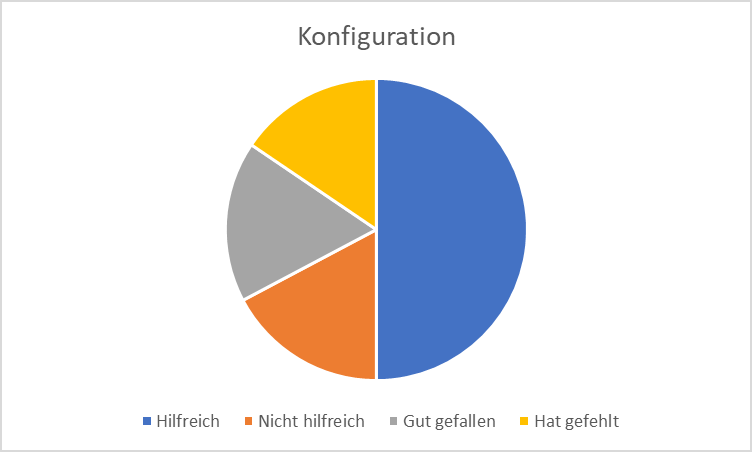
\includegraphics[width=1\textwidth]{pictures/diagramme/aussagenkonfig}
\caption{Anteile der Aussagen, die Probanden in der abschließenden Fragerunde bezüglich des Konfigurationsprinzip äußerten.}
\label{aussagensichtb}
\end{figure}


\paragraph{Hilfreich}Die Hälfte der Probanden empfanden besonders die zeitliche Darstellung als hilfreich. Ein Proband beschrieb, dass das Zusammenbringen der Einstellungen und des zeitlichen Ablaufs der Übersicht beiträgt. Ein weiterer ging darauf ein, dass der Zeitstrahl gut interpretierbar ist. Auch da dieser konsistent nach rechts fortlaufend ist. Knapp achtunddreißig Prozent der Probanden äußerten auch, dass die Darstellung generell als übersichtlich empfunden wurde. Weitere Aussagen bekräftigen diese Äußerung. So wurde das System generell als benutzerfreundlich eingestuft. Unter anderem wurde dies durch die Anlehnung an das bekannte Material Design von Google begründet. Auch wurde angemerkt, dass wichtige Informationen und Funktionen im Vordergrund stehen und auch auf die Funktionen reduziert wurde, die für einen entsprechenden Chatbot benötigt werden. Des weiteren wurden die zeitlichen Abhängigkeiten als gut einsehbar empfunden. Hierzu gab es zwei Aussagen die dies hervorhoben. Zwei Anmerkungen bezogen sich auf die farbliche Kodierung der Trigger-Arten. Die Unterscheidung dieser innerhalb der zeitlichen Darstellung wurde positiv empfunden. Auch die Auflistung der Konversationen innerhalb der Darstellung wurde positiv angemerkt. Die Suchfunktion erleichtere das Finden einzelner Konversationen. Dies äußerten ebenfalls zwei Probanden.


\paragraph{Nicht hilfreich}Zwei Probanden konnten keine Aussage darüber treffen, was sie als nicht hilfreich empfanden. Vier weitere Probanden hingegen gaben an, dass die Legende, die in der Darstellung der Umsetzung vorfanden, eher irritierend wahrnahmen. Hier fehlte ihnen eine ausführliche Erklärung der farblichen Kodierung. Außerdem wurden die Icons, die in der zeitlichen Übersicht auftauchten,in der Legende vermisst. Ein weiterer Proband wünschte sich die Möglichkeit, die Konversationen innerhalb der zeitlichen Darstellung klickbar zu gestalten, um daraufhin beispielsweise die Trigger-Einstellungen der entsprechenden Konversation zu öffnen. Des weiteren irritierte einen Probanden die Aufteilung zwischen den Abhängigen Konversationen.

\paragraph{Gut Gefallen} Auf die Frage, was den Probanden an der Umsetzung besonders gut gefallen habe, konnte ein Proband keine Aussage treffen. Siebenunddreißig Prozent der Probanden hingegen gaben an, dass ihnen die zeitliche Darstellung der Konversationen besonders gut gefiel. Ein Proband merkte dabei an, dass auf diese Weise die Belastung der Therapie-Teilnehmer auf einen Blick  einsehbar ist. Auch wurden von weiteren siebenunddreißig Prozent angegeben, dass die Konversation und Trigger gut ineinander greifen. Gefühlt müssen weniger Einstellungsschritte vorgenommen werden und der Fluss dieser wirkt klarer und konsistenter.

\paragraph{Gefehlt} Drei Probanden konnten keine Aussage darüber treffen, was sie an dieser Form der Umsetzung vermisst haben. Fünfundfünzig Prozent der genannten Punkte gingen auf fehlende Hilfestellungen ein. Zum einen wünschen sich die Probanden Anleitungen beziehungsweise Tutorials zur Einführung. Zum anderen vermissten sie Tooltips, die Informationen zu verschiedenen Funktionen und Elementen offenlegen. Desweiteren wünschen sie sich eine Funktion hinter den einzelnen Elementen innerhalb der Zeitdarstellung. Zwei Probanden beschrieben, dass ihnen eine hinterlegte Funktion fehlt, die durch das Anklicken eines solchen Elements ausgelöst wird. Gewünscht wurde hier das Öffnen der Einstellungsmöglichkeiten oder Anzeigen von zugehörigen Informationen der Trigger-Einstellungen. Zusätzlich wünschten sich zwei weitere Probanden eine ausführlichere Legende die mehr Informationen über die Farben und Symbole bietet.

\subsection{Evaluationsergebnis der Sprünge}
Zunächst werden die zugehörigen Daten der Methode, die im \emph{TherapyBuilder} zum Einsatz kam, untersucht. Wie in Abbildung \ref{spruenge} zu erkennen ist, wird der Konversationsverlauf, ähnlich eines herkömmlichen Chatverlaufs bekannter Technologien, versetzt dargestellt. 

\begin{figure}[h]
\centering
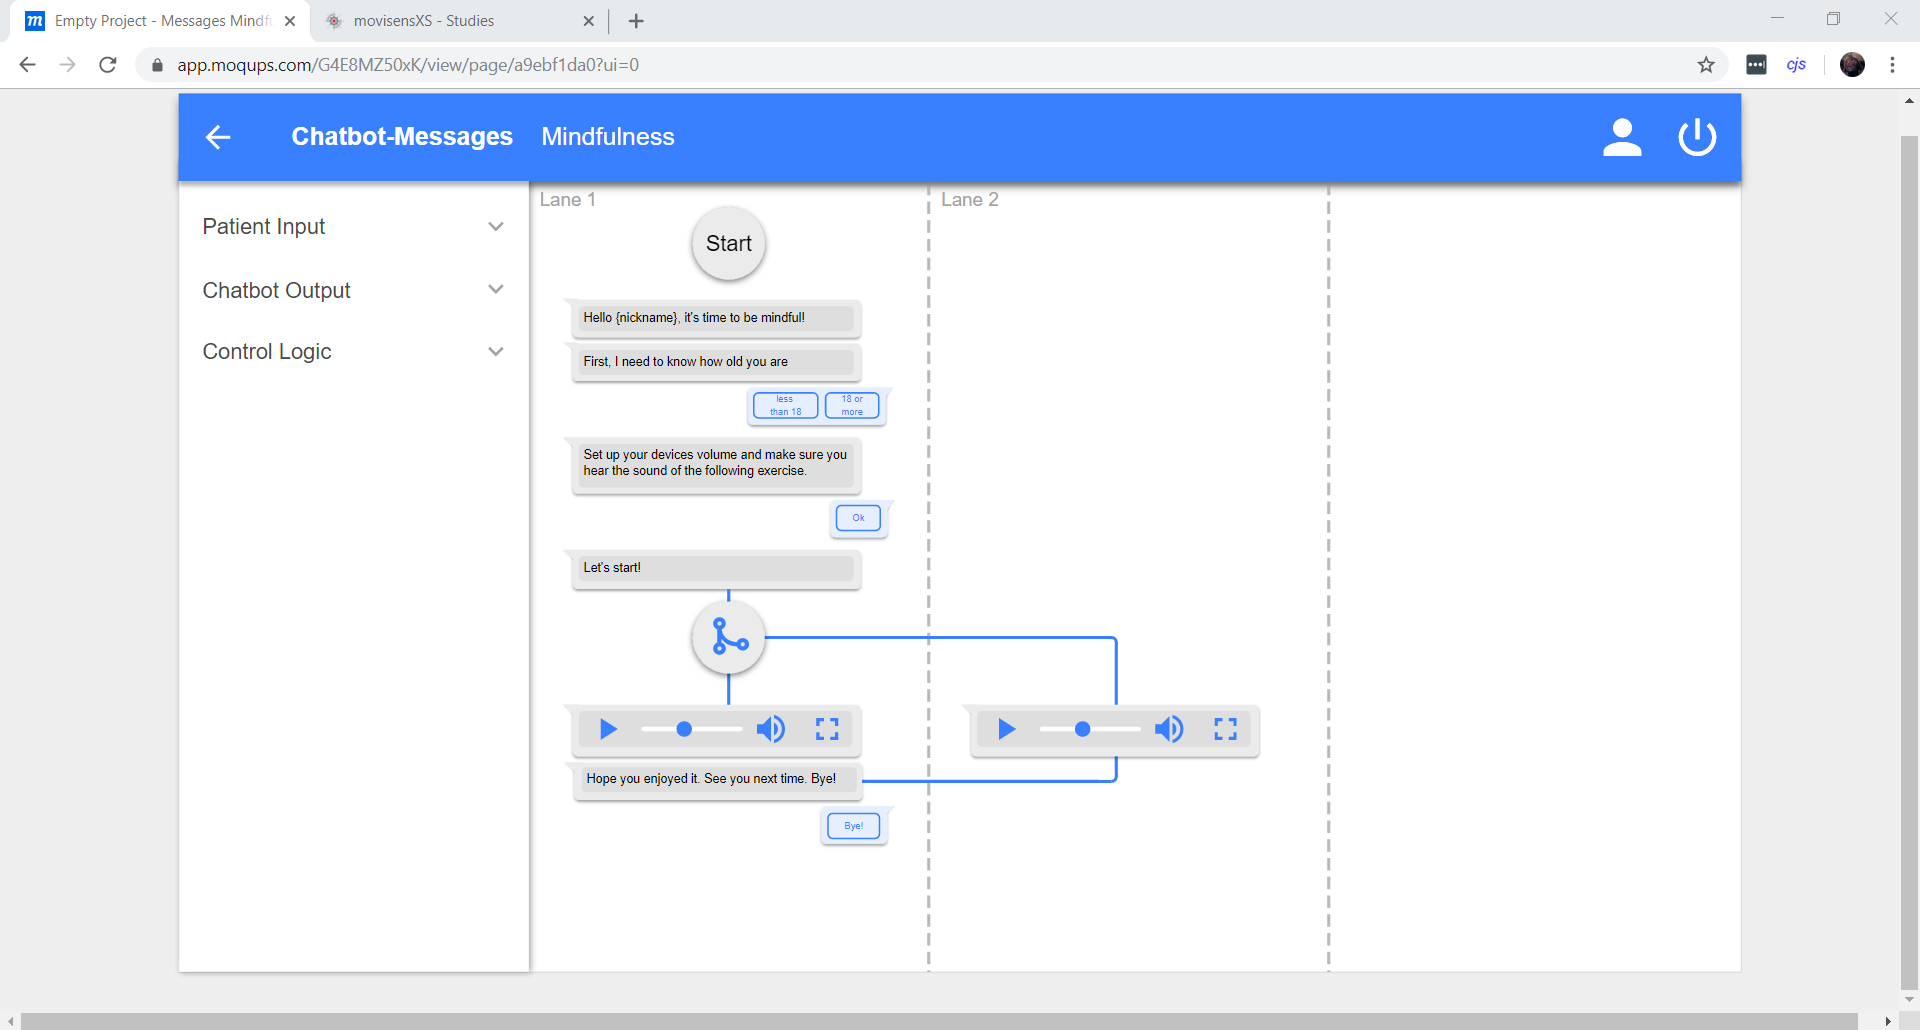
\includegraphics[width=1\textwidth]{pictures/spruenge}
\caption{Der Prototyp \emph{TherapyBuilder} stellt alternative Gesprächsverläufe als Sprünge dar. Diese werden mit einem runden Element und einem entsprechenden Icon versinnbildlicht. Anhand der hinterlegten Bedingungen wird im Gesprächsverlauf entschieden, welchen Gesprächsverlauf dem Nutzern dargeboten wird. Dabei verweist der Sprung auf verschiedene Lanes die den entsprechenden Verlauf beinhalten.}
\label{spruenge}
\end{figure}

Nachfolgend werden die erhobenen Daten beschrieben, die bezüglich der betrachteten Sprung-Methodik erhoben wurden. Zunächst werden die Ergebnisse des Zwischenfragebogens, anschließend die Ergebnisse der Abschlussfragerunde dargestellt.

\subsubsection{Zwischenfragebogen}
Die Ausgaben des Chatbots werden in einer grauen Sprechblase abgebildet. Die Sprechblase ist nach links orientiert ausgerichtet. Die Eingabeformate des Anwenders werden in einer blauen Sprechblase dargestellt. Diese sind nach rechts orientiert. Der Gesprächsverlauf wird in sogenannten \emph{Lanes} dargestellt. Zunächst wird dieser innerhalb einer \emph{Lane} angelegt. Wird ein alternativer Gesprächsverlauf dargeboten, so wird dies durch eine Condition, in Form eines runden Elements, angedeutet. Dieses runde Element kann entsprechend der Bedingung eingestellt werden und bestimmt, in welcher \emph{Lane} der alternative Gesprächsverlauf weitergeführt wird. 

Hinsichtlich der Darstellung der Konversationen beurteilten die Probanden diese als voll und ganz verständlich. Dies lässt sich auch in den Freitexten der Probanden wiederfinden. Knapp achtundachtzig Prozent der Aussagen äußern sich positiv über die Darstellung der Konversationen. So gefällt im allgemeinen die zeitliche Abfolge, die Gestaltung wie auch die Übersichtlichkeit. 

Die Einstellungsmöglichkeiten der Konversationen empfanden die Probanden im Schnitt als voll und ganz verständlich. Sie tendierten leicht zu zumeist verständlich. Ein Proband äußerte sich auch positiv über die Möglichkeit, die Konversation in dem dargestellten Ablauf zu bearbeiten. Ein weiterer merkte die vielen Einstellungsmöglichkeiten an, die dennoch nicht visuell erschlagen.

Bezüglich des Konversationsverlaufs und dessen Übersichtlichkeit äußerten die Probanden, dass diese im Schnitt als sehr gut empfunden wird. Dabei gibt es eine sehr leichte Tendenz zu \emph{als gut empfunden}. Die Freitext-Aussagen bekräftigen dies. Hier wird vermehrt auf die Übersichtlichkeit eingegangen. Die Hälfte der Probanden-Aussagen gaben dies unter den Punkten an, die ihnen am System am besten gefallen haben. Die Hälfte der Probanden gaben unter diese Punkt allgemein an, dass ihnen die Darstellung der Konversationen gefallen hat.

Antwortoptionen eines Konversationsverlaufs wurden im Allgemeinen als Übersichtlich wahrgenommen. Im Schnitt wurde diese als sehr gut bewertet. Keiner der Probanden ging innerhalb der Freitext-Angaben weiter darauf ein.

Verzweigungen innerhalb eines Konversationsverlaufs wurden ebenfalls im Schnitt als sehr gut verständlich empfunden. Es ließ sich hier eine leichte Tendenz zur Einschätzung \emph{gut verständlich} erkennen. Ein Proband schrieb, dass die Konditionen Sinn ergeben. Eine weitere Anmerkung weißte allerdings auf die Befürchtung hin, dass die Lane-Anordnung, die bei einer Verzweigung entsteht, bei mehr als drei Verzweigungen kompliziert werden könnte. Außerdem konnte ein Proband aus der Grafik nicht genau ableiten, welche Bedingungen und Entscheidungen zusammenhängen. 

Die Werkzeugpalette zur Erstellung des Konversationsverlaufs wurde im Schnitt als sehr Übersichtlich, mit einer Tendenz zu gut Übersichtlich, wahrgenommen. Hier wurde von einem Probanden angemerkt, dass viele Einstellungsmöglichkeiten angeboten werden, ohne mit diesen visuell zu erschlagen. Auch die Aussage, dass die Konditionen Sinn ergeben, bekräftigen das Ergebnis der Fragebogen-Auswertung. 

\subsubsection{Abschlussfragerunde}
Innerhalb der Abschlussfragerunde äußerten die Probanden insgesamt 41 Punkte über die Verwendung und Darstellung von Sprüngen innerhalb eines Konversationsverlaufs. Neununddreißig Prozent der genannten Punkte beziehen sich auf die Nachfrage, was die Probanden als besonders Hilfreich empfanden. Knapp fünfzehn Prozent der Punkte nannten die Probanden auf die Frage, welche Eigenschaften sie als nicht hilfreich erlebten. Vierundzwanzig Prozent der angegebenen Punkte ordnen sich der Aufgabe zu, Eigenschaften zu nennen, die den Probanden gut gefallen haben. Die restlichen zweiundzwanzig Prozent beziehen sich auf die Eigenschaften, die von den Probanden bei diesem Konzept vermisst haben.  

\begin{figure}[h]
\centering
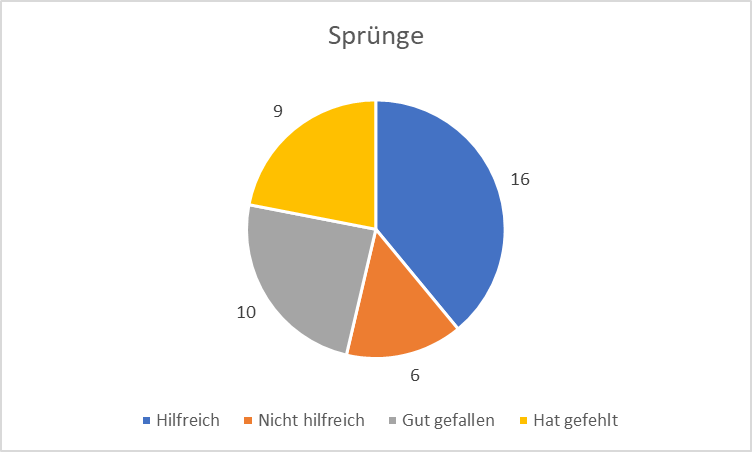
\includegraphics[width=1\textwidth]{pictures/diagramme/aussagenspr}
\caption{Anteile der Aussagen, die Probanden in der abschließenden Fragerunde bezüglich der Verwendung von Sprüngen äußerten.}
\label{aussagensichtb}
\end{figure}
 

\paragraph{Hilfreich} Siebenunddreißig Prozent der Aussagen nannten die gute Sichtbarkeit die in der Darstellung der Sprünge geboten wird. So ist, nach Probandenaussagen, auf einen Blick sichtbar wo und wann der Sprung stattfindet. Fünfundzwanzig Prozent sagen aus, dass der Gesprächsverlauf klarer strukturiert ist. Neben diesen Äußerungen wurden noch weitere Punkte geäußert. Die Bedeutung des Konzepts und dessen Darstellung ist offensichtlicher, die Einteilung in Lanes geben dem Gesprächsverlauf Struktur und die Darstellung der Konversation ist klar und verständlich dank der Verwendung eines gewohnten Formats. Diese Äußerungen machen je dreizehn Prozent aller getroffenen Aussagen zur Frage, was als Hilfreich empfunden wurde, aus.

\paragraph{Nicht hilfreich}Die Hälfte der Probanden konnten auf die Frage, welche Eigenschaften des Konzepts sie als nicht hilfreich einstufen, keine Aussage treffen. Zur Darstellung des Bauelements, welches zur Konfiguration der Sprünge dient, wurden dreiunddreißig Prozent der Aussagen getroffen. Hier wurde die Befürchtung geäußert, dass bei steigender Komplexität des Konversationsverlaufs, die Übersicht verloren geht. Weitere dreiunddreißig Prozent sprachen die Einstellung des Elements an. So benötigt es für den Umgang damit erst ein Gefühl. Zwei weitere Punkte sprechen einmal das Wording und den Rücksprung zur ersten Lane an. Beides wurde als irritierend bezeichnet.

\paragraph{Gut Gefallen}Auf die Frage hin, welche Eigenschaften des Konzepts ihnen besonders gut gefallen hat, konnten drei Probanden keine Antwort finden. Dreißig Prozent der Äußerungen sagen aus, dass die Lanes besonders gut gefallen haben. Weitere dreißig Prozent beziehen sich auf die Sprünge. Diese wurden als klar verständlich wahrgenommen. Zwanzig Prozent nennen die zeitliche Anordnung der Konversationselemente. Ein weiterer Punkt bezieht sich auf den Zustand der Werkzeugpalette, sobald die Konversation-Ansicht aufgerufen wird. Auch nannte ein Proband die Einstellungs-möglichkeiten des Sprung-Elements.

\paragraph{Gefehlt}Vier Probanden sagten aus, sie hatten nicht den Eindruck, dass sie an der Umsetzung des Konzepts etwas vermisst haben. Die andere Hälfte hingegen äußerte sich zu sechs verschiedenen Punkten. So geben dreiunddreißig Prozent der Aussagen an, dass Anleitungen, beispielsweise in Form von Tooltips, vermisst wurden. Weitere zweiundzwanzig Prozent äußerten sich zur Darstellung des Rücksprungs. Hier wünschten sich zwei Probanden eine andere Darstellungsform. Ein Proband gab an, dass dieser sich einen Entwicklermodus für Power-User wünschen würde. Weitere Einzelnennungen beziehen sich auf eine bessere farbliche Unterscheidung der Elemente, mehr Bearbeitungs- und Gestaltungsfreiraum und der fehlenden Vorstellung, wie eine weitaus komplexere Konversation aussehen könnte.    

\subsection{Evaluationsergebnis der Sichtbarkeitsregeln}
Die Sichtbarkeitsregeln unterscheiden sich maßgeblich von dem Konzept der Sprünge, die zuvor betrachtet wurden. Die Sichtbarkeit eines Elements, welches einen Teil einer Konversation darstellt, wird anhand eines Icons, in Form eines Auges, angedeutet. Die Einstellungsmöglichkeit der Sichtbarkeit erscheint, sobald der Nutzer den Mauszeiger über eines der Elemente bewegt. Anschließend kann, durch ein Klick auf das Auge, die Einstellung der Sichtbarkeitsregel vorgenommen werden. Hier wird entschieden, für welche Gruppe das entsprechende Element im Gesprächsverlauf erscheint. Diese Einstellung wird anhand einer Regel festgelegt. Diese Regel prüft ein oder mehrere Variablen ab. Wurde eine solche Regel einem Element hinterlegt, so erscheint an diesem das Augensymbol dauerhaft, wie in Abbildung \ref{sichtbarkeit} zu sehen ist. Darüber hinaus werden die Dialoge des Konversationsverlaufs anhand von Forms zusammengesetzt. Diese beinhalten entweder nur einen Chatbot-Output oder Chatbot-Output und Input des Nutzers. 

\begin{figure}[h]
\centering
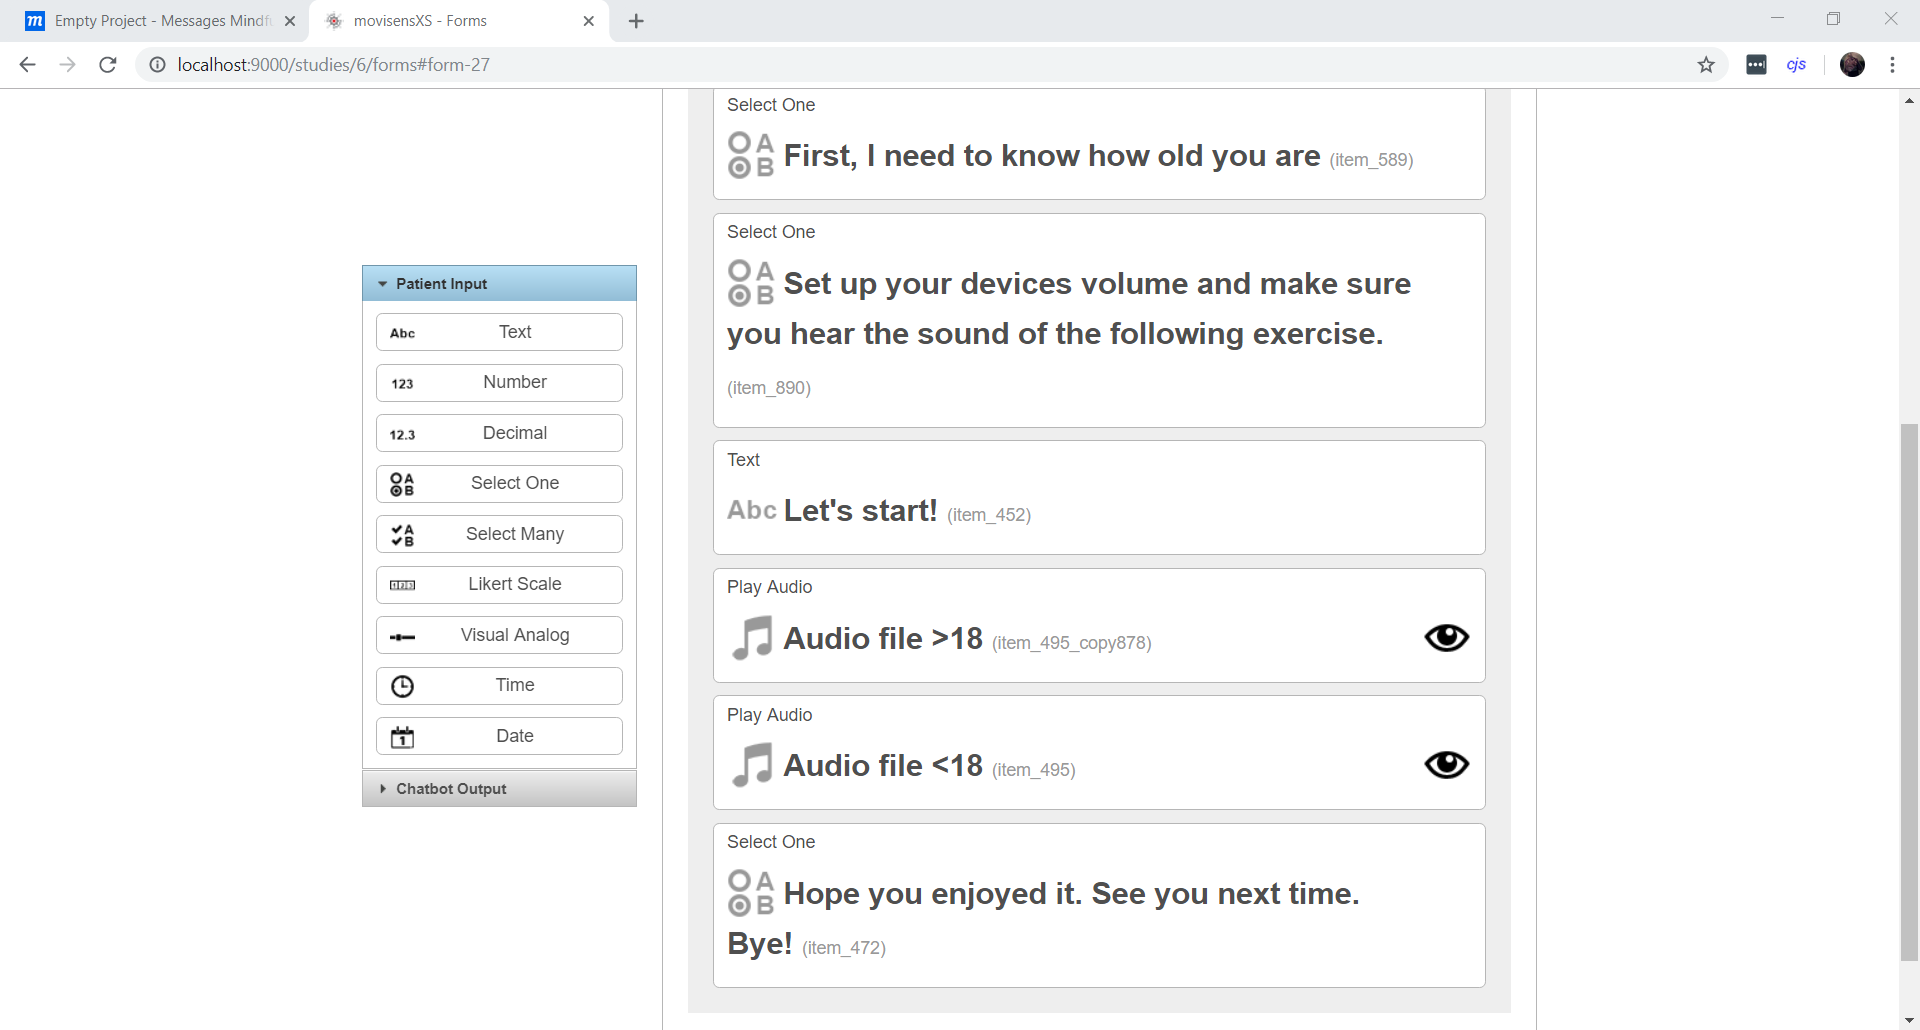
\includegraphics[width=1\textwidth]{pictures/sichtbarkeit}
\caption{Anteile der Aussagen, die Probanden in der abschließenden Fragerunde bezüglich der Sichtbarkeit äußerten.}
\label{sichtbarkeit}
\end{figure}

Nachfolgend werden die erhobenen Daten beschrieben, die bezüglich der betrachteten Sichtbarkeitsregeln erhoben wurden. Zunächst werden die Ergebnisse des Zwischenfragebogens, anschließend die Ergebnisse der Abschlussfragerunde dargestellt.

\subsubsection{Zwischenfragebogen}
Dieses Konzept wurde ebenfalls von den Probanden bewertet. Aus der Bewertung lassen sich folgende Aussagen treffen. 

Auf Basis der Sichtbarkeitsregel und dem Design des Konversationsverlaufs wurde die Darstellung der Konversationen generell als zumeist verständlich bewertet. Es lässt sich eine leichte Tendenz erkennen, die angibt, dass die Darstellung zum Teil verständlich ist. Die Probandenaussagen der Freitexte untermauern die Bewertung. Es wurden bezüglich der Darstellung keine Punkte genannt, die den Probanden besonders positiv hervorstach. Hingegen wurden mehrere Aussagen getroffen, welche die Darstellung der Konversationen bemängeln. Etwas mehr als sechzig Prozent der Nutzer haben sich diesbezüglich negativ geäußert.

Die Einstellungmsöglichkeiten der Konversationen wurde von den Probanden ebenfalls als zumeist verständlich, mit leichter Tendenz zu zum Teil verständlich, wahrgenommen. Hier wurde in knapp achtunddreißig Prozent der Aussagen die Vielfalt der Einstellungsmöglichkeiten positiv hervorgehoben. Auch die Kategorisierung der Einstellungsmöglichkeiten wurde einmal positiv erwähnt. Hingegen wurde ebenfalls in achtunddreißig Prozent der Aussagen die Unterscheidbarkeit zwischen Chatbot-Output und Patient-Input Elementen, innerhalb des Werkzeugkastens, bemängelt. Diese unterscheiden sich kaum. 

Als gut, mit starker Tendenz zu eher gut, wurde im Schnitt die Übersichtlichkeit des Konversationsverlaufs bewertet. Vier der Freitextaussagen bemängeln die Übersicht der Konversationen. Zum einen sei der zeitliche sowie der generelle Verlauf schwer nachvollziehbar.

Die Übersichtlichkeit der Antwortoptionen innerhalb eines Konversationsverlauf wurden von den Probanden im Schnitt als gut empfunden. Die durchschnittliche Bewertung weist dabei eine starke Tendenz zu \emph{eher gut} auf. Dies lässt sich auch in den schriftlichen Aussagen der Probanden wiederfinden. Vier Aussagen äußern sich negativ zur Darstellung des Verlaufs. Keine Aussage geht speziell auf die Antwortoptionen ein. 

Als eher gut bewerteten die Probanden im Schnitt die Verständlichkeit der Verzweigungen innerhalb einer Konversation. Hierzu passen die Freitext-Aussagen der Probanden, die angaben, dass die Übersicht des zeitlichen Verlaufs fehle und somit für diese Probanden eher schwer nachvollziehbar ist. Diese Aussage trafen fünfzig Prozent. Ein Proband wies außerdem darauf hin, dass ihm unklar ist, woher die Variable stammt, die für die Verzweigung überprüft wird. 

Im Schnitt bewerteten die Probanden die Übersichtlichkeit der Werkzeugpalette zur Erstellung des Konversationsverlaufs als gut. Auch hier zeigte sich eine starke Tendenz zur schlechteren Bewertung. Hier merkte ein Probanden an, dass der Zustand der Werkzeugpalette beim Öffnen des Konversationsreiters, hinderlich ist. Die Einstellungsmöglichkeiten des Chatbot-Outputs sind durch diesen leicht zu übersehen. 

\subsubsection{Abschlussfragerunde}
Insgesamt wurden einunddreißig Aussagen zur Umsetzung von Sichtbarkeitsregeln genannt. Neunzehn Prozent beziehen sich auf die Erläuterungen der Probanden, was sie als besonders Hilfreich wahrgenommen haben. Einundfünfzig Prozent gingen auf die Frage \emph{Was haben Sie als weniger oder gar nicht hilfreich empfunden?} ein. Auf die Nachfrage, was an diesem Konzept besonders gut gefallen hat, konnte kein Proband eine Angabe äußern. Neunundzwandzig Prozent der Aussagen hingegen, erläuterten welche Eigenschaften an diesem Konzept vermisst wurden.


\begin{figure}[h]
\centering
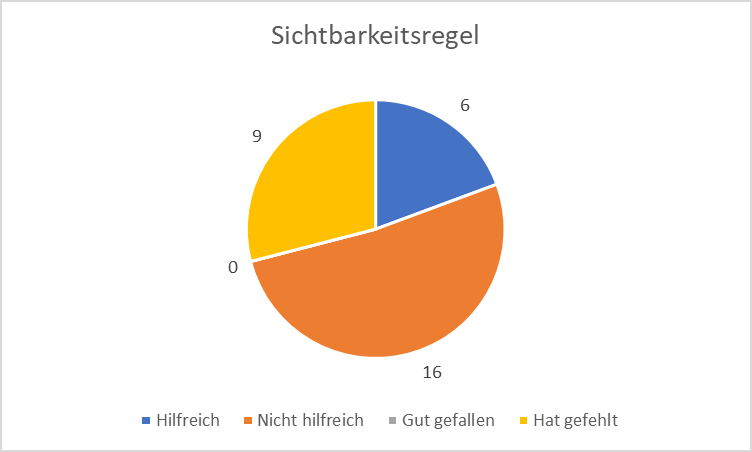
\includegraphics[width=1\textwidth]{pictures/diagramme/aussagensichtb}
\caption{Anteile der Aussagen, die Probanden in der abschließenden Fragerunde bezüglich der Sichtbarkeitsregeln äußerten.}
\label{aussagensichtb}
\end{figure}

\paragraph{Hilfreich}Die Hälfte der Probanden konnten keine Eigenschaften finden, die sie als besonders Hilfreich wahrgenommen haben. Zwei Probanden äußerten sich positiv über die \emph{Drag and Drop}-Funktion der Form-Elemente zur Erstellung des Konversationsverlaufs. Der Umgang mit dem Auge fiel zwei Probanden leicht, da sie eine ähnliche Funktionsweise bereits durch andere Programmen, wie \emph{REDCap}, kennengelernt haben. Zum Auge wurde ebenfalls genannt, dass daraus der Kontext \emph{Irgendetwas sehen} klar hervorgeht. Ein Proband empfand das Bearbeiten eines Form-Elements durch Doppelklick, als besonders Hilfreich.

\paragraph{Nicht hilfreich}Als nicht hilfreich wurde der hohe Kognitive Aufwand angegeben, der mit der Darstellung des Auges einhergeht. Einunddreißig Prozent der Aussagen bezogen sich auf diesen und nannten als Gründe die Unübersichtlichkeit, sowie die Notwendigkeit die Regeln und Abfolge im Gedächtnis behalten zu müssen. Weitere fünfzig Prozent der Aussagen gaben an, dass die Augen-Metapher in der verwendeten Form nicht sehr zugänglich ist. Es geht unter, wird leicht übersehen oder vergessen, das gewählte Icon in Form eines Auges ist eher irritierend und die Funktion wird erst klar, sobald es angeklickt wurde. Weiter Punkte die außerdem einzeln genannt wurden, gingen auf die fehlende Bedienungsanleitung, das leicht zu übersehende Löschen-Symbol innerhalb der Konfiguration der Sichtbarkeitsregel, sowie die generell als lieblos und wenig intuitiv empfundene Gestaltung des Konzepts ein. 

\paragraph{Gut Gefallen}Wie bereits beschrieben, konnte kein Proband, auf die Bitte zu erläutern was diesen besonders gut gefallen hat, eine Aussage tätigen.

\paragraph{Gefehlt}Folgende Eigenschaften haben die Probanden, laut Aussage, an diesem Konzept vermisst: eine Bedienungsanleitung, eine bessere Übersicht über den Konversationsverlauf, sowie eine Übersicht der vorhandenen Variablen. Knapp Sechsundfünfzig Prozent der Aussagen äußerten den Wunsch nach einer Bedienungsanleitung. Ungefähr Dreiunddreißig Prozent gingen auf die fehlende Übersicht ein. Ein Proband wünschte sich die Variablenübersicht. Drei Probanden konnten nicht Erläutern, welche Eigenschaften sie vermisst haben.
